\chapter{Entwicklung}
\section{Igel Informationen}
Da das Spiel einen Einblick in die Lebensweise eines Igels geben soll, mussten im ersten Schritt die dazu nötigen Informationen eingeholt werden. Dazu wurde zum einen im Internet danach gesucht und Magdalena Bienefeld hatte sich mit Jana Zwanziger aus Führt getroffen, die eine Pflegeeinrichtung für Igel führt. Dadurch konnten Informationen aus erster Hand gesammelt werden. \cite{Igelrettung} 

Um Igel zu unterstützen, soll man ihnen als Nahrungsmöglichkeit keine Milch zur Verfügung stellen, sondern Wasser. Igel können Milch nicht verarbeiten, da sie Laktoseintolerant sind. Am liebsten Fressen sie Käferlarven, Raupen oder Regenwürmer. Zur Unterstützung der  Nahrungsfindung kann der Mensch ihnen Katzenfutter oder Eier zur Verfügung stellen. Auf keinen Fall dürfen sie Äpfel, Nüsse oder andere Speisereste erhalten. 

Neben den natürlichen Fressfeinden wie dem Dachs, dem Uhu oder dem Fuchs sind in den letzten Jahren durch den technologischen Fortschritt die Straßen mit den Autos und vor allem die Rasenmäherroboter hinzugekommen, da diese meistens auch dann in den Gärten fahren, wenn Igel auf ihren Streifzügen sind. Durch den Verlust von naturnahen Gärten verlieren Igel immer weiter ihren Lebensraum. 

Igel halten auch einen Winterschlaf, da sie in den Monaten zu wenig Nahrung finden würden. Abhängig von der Witterung suchen sie sich gegen November einen Unterschlupf. Während des Schlafs fahren Igel ihre Körpertemperatur und  den Stoffwechsel auf ein Minimum herunter. Vor ihren Schlaf fressen sie sich genug Fettreserven an. \cite{Igel_Infos_1, Igel_Infos_2}

Diese Elemente wurden in Form von den Stationen im  VR-Spiel umgesetzt.


\section{Soundeffekte}
Nachdem das erste Konzept der Welt festgehalten wurde und die Rahmenbedingungen festgestanden waren, ging es auf die Suche nach Soundeffekten. Bei der Suche nach möglichen Audiodateien war es insbesondere wichtig auf die Lizenzen zu achten. So wurde hauptsächlich Musik mit der CC0 Lizenz verwendet. Diese Lizenz ermöglicht es, ohne den Urheber zu kontaktieren oder zu erwähnen seine Arbeit zu verwenden. Zudem ist es gestattet, dass die Audiodateien auch bearbeitet werden. \cite{CC0_Lizenz, freesound, opengameart} 

Ein Teil der Musik wurde mit der open-source Software Audacity geschnitten. Somit konnten sie auf die passende Länge gekürzt werden oder aus einem längeren Soundtrack der interessierende Teil herausgeschnitten werden. 

Die im Spiel zu hörenden Texte wurden durch Saniye Ogul aufgenommen und eingespielt. Zudem hat sie die gefundenen und geschnittenen Soundeffekte bei den einzelnen Stationen implementiert.


\section{Station 7: Rasenmäher}
\subsection{Bezier-Kurve}
Eine Kurve im $\mathbb{R}^3$ ist durch eine Abbildung 
\begin{align}
	\label{KurveimRaum}
	c:[a,b] \mapsto \mathbb{R}^3, ~ t \mapsto \begin{pmatrix}
		x(t)\\
		y(t)\\
		z(t)
	\end{pmatrix}
\end{align}
gegeben. Der Parameter t kann dabei als Variable über der Zeit interpretiert werden und die Kurve wird somit im Intervall $t\in[a, b]$ durchlaufen.

Zu jedem Zeitpunkt soll $b(t)$ eine gewichtete Summe der Kontrollpunkte der Kurve sein:
\begin{align}
	b(t) = B_0(t)b_0 + B_1(t)b_1 + B_2(t)b_2+B_3(t)b_3.
\end{align}
Es soll folgendes gelten:
\begin{itemize}
	\item $B_0(t) + B_1(t) + B_2(t) + B_3(t) = 1 ~ \forall ~ t \in [a, b]$
	\item $B_i \geq 0 ~ \forall ~ t \in [a, b], ~ i=0, 1, 2, 3$.
	\item $t=0 ~ ist ~ B_0^3(0)=1 ~ und ~ B_1^3(0)=B_2^3(0)=B_3^3(0)=0$ \\$\Rightarrow b(0)=b_0$
	\item $t=1 ~ ist ~ B_3^3(1)=1 ~ und ~ B_0^3(1)=B_1^3(1)=B_2^3(1)=0$ \\$\Rightarrow b(1) = b_3$
\end{itemize}

Für eine kubische Bezier-Kurve $b(t)$ werden die Bernstein-Polynome als Gewichtsfunktion verwendet. Diese haben folgende Gestalt und erfüllen die oben genannten Eigenschaften: \cite{BezierKurven_Theorie}
\begin{align}
	B_k^3 = \begin{pmatrix}
		3\\
		k
	\end{pmatrix} X^k(1-X)^{3-k}
\end{align}


\subsection{Implementierung}
\begin{figure}[H]
	\centering
	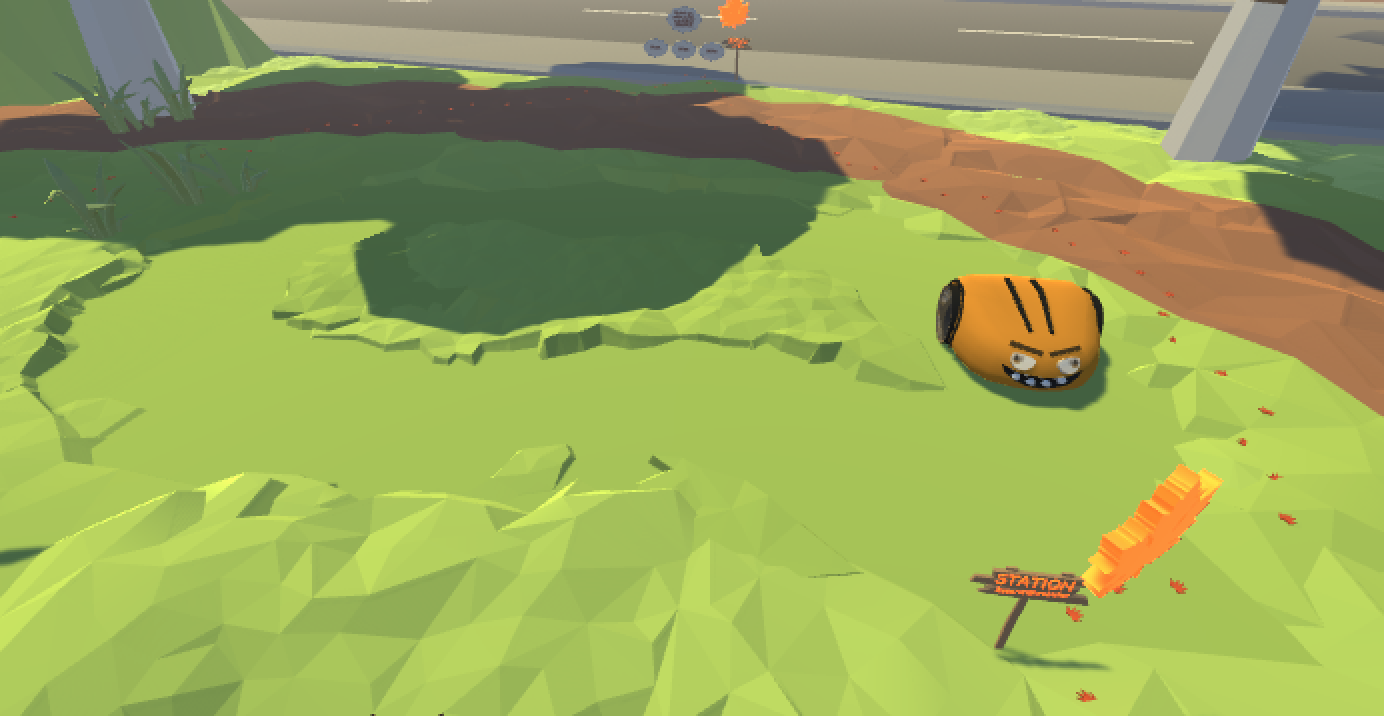
\includegraphics[width=0.675\linewidth]{station_robot.png}
	\caption[Übersicht über die Rasenmäher Station]{Übersicht über die Rasenmäher Station. Quelle: Eigene Aufnahme}
	\label{fig:station_robot}
\end{figure}

In \autoref{fig:station_robot} ist die Übersicht über den Aufbau der Station gegeben. Die Landschaft und der Rasenmäherroboter wurden von Magdalena Bienefeld entworfen. Mithilfe meines Strecken Skripts wurde dem Roboter leben eingehaucht. 

Dazu kann mit den Ankerpunkten 2 und 3 die Streckenform angepasst werden und mit den Ankerpunkten 1 und 4 der Start- und Zielpunkt der Kurve festgelegt werden. Durch aneinanderreihen dieser Kurven fährt der Roboter die geschlossene Kurve ab. Dabei ist zu beachten, dass der Punkt 1 von Kurve A mit dem Punkt 4 von Kurve B und Punkt 4 von Kurve A mit dem Punkt 1 von Kurve B zusammenfallen. Falls dies nicht beachtet wird, kommt es zu Sprüngen in der Strecke. Die Strecke wurde nach dem Vorbild aus einem Video entworfen. \cite{Unity_BezierCurve_Youtube}



\subsection{Problematik}
%Bild einfügen
%Probleme -> ungerade ursp. Fläche --> ging nicht mehr
Einer der ersten Entwürfe der Karte hatte über die gesamte Fläche Unebenheiten. Dies führte allerdings durch die implementierte Gestalt der Bézierkurve dazu, dass der Roboter durch diese Unebenheiten hindurch fährt. 

In ersten Gedanken sollte das Hinzufügen einer Rigidbody Komponente und das Einschalten der Gravitation das Problem beheben. Es sollten die Koordinaten in der xz-Ebene mit der Kurve berechnet werden und der Roboter durch die Gravitation an den Boden gezogen werden. Ein Collider sollte verhindern, dass das Objekt durch die Landschaft fällt. 

Jegliche Versuche führten allerdings nur zu dem Ergebnis, wie es in \autoref{fig:robot_problem} dargestellt ist. Das Problem wurde durch das Anpassen der Landschaft umgangen. Im neuesten Entwurf sieht die abgefahrene Strecke des Roboters nach einer gemähten Wiese aus.

\begin{figure}[H]
	\centering
	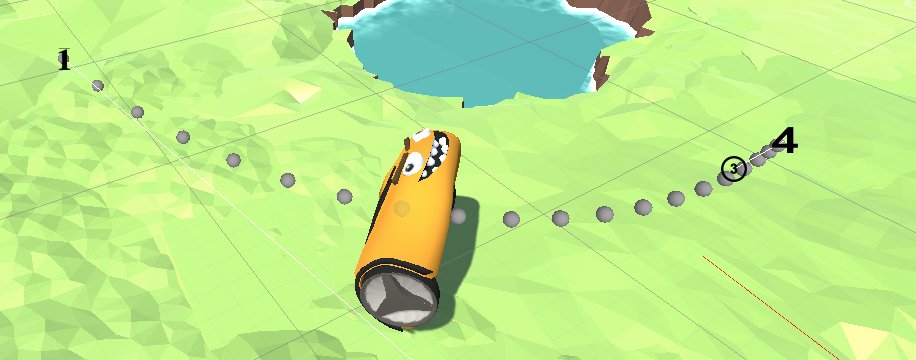
\includegraphics[width=0.5\linewidth]{robot_problem.png}
	\caption[Darstellung des Problems der unebenen Fläche]{Darstellung des Problems der unebenen Fläche. Quelle: Eigene Aufnahme}
	\label{fig:robot_problem}
\end{figure}



\section{Station 8: Straße}
\subsection{Auto Design}
\begin{figure}[H]
	\centering
	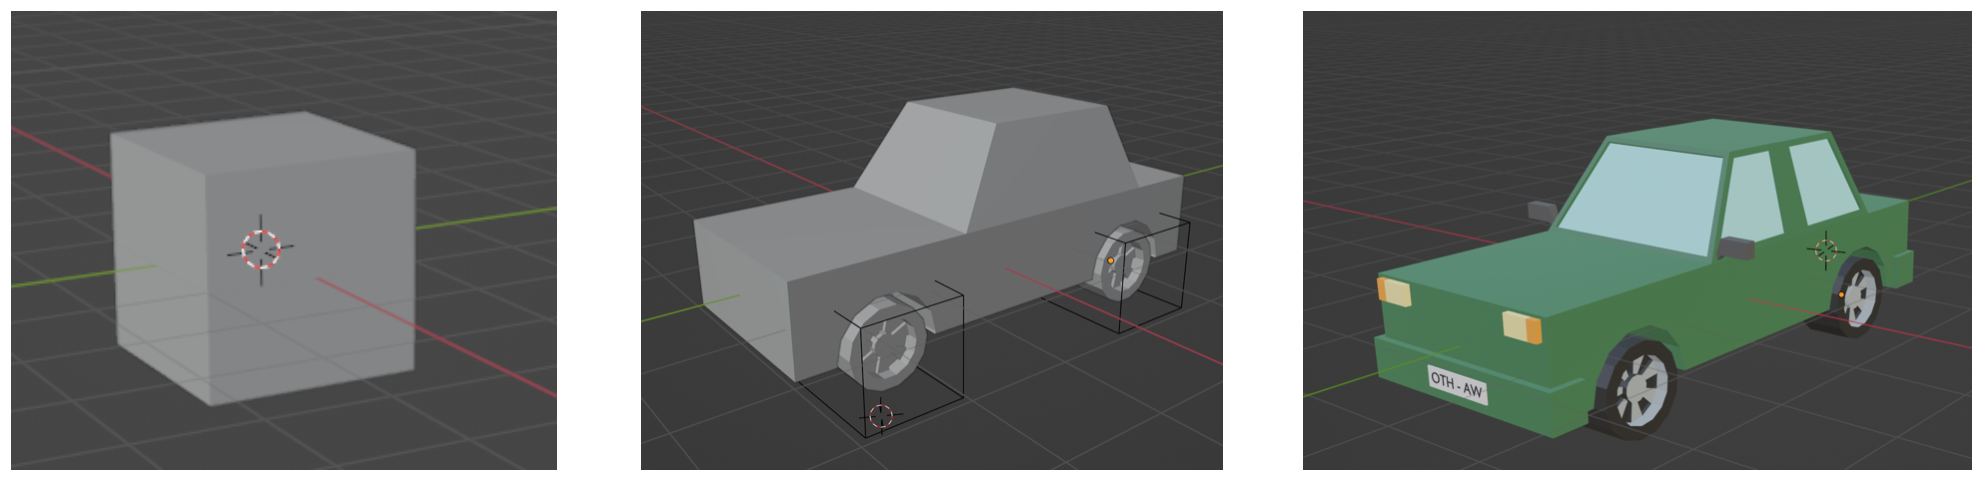
\includegraphics[width=0.8\linewidth]{Development_Car.png}
	\caption[Entwicklungsprozess des Autos mit Blender]{Entwicklungsprozess des Autos mit Blender. Links: Ausgangsobjekt, Mitte: Zwischenstand, Rechts: Fertige Objekt. Quelle: Eigene Aufnahme}
	\label{fig:development_car}
\end{figure}

\begin{figure}[H]
	\centering
	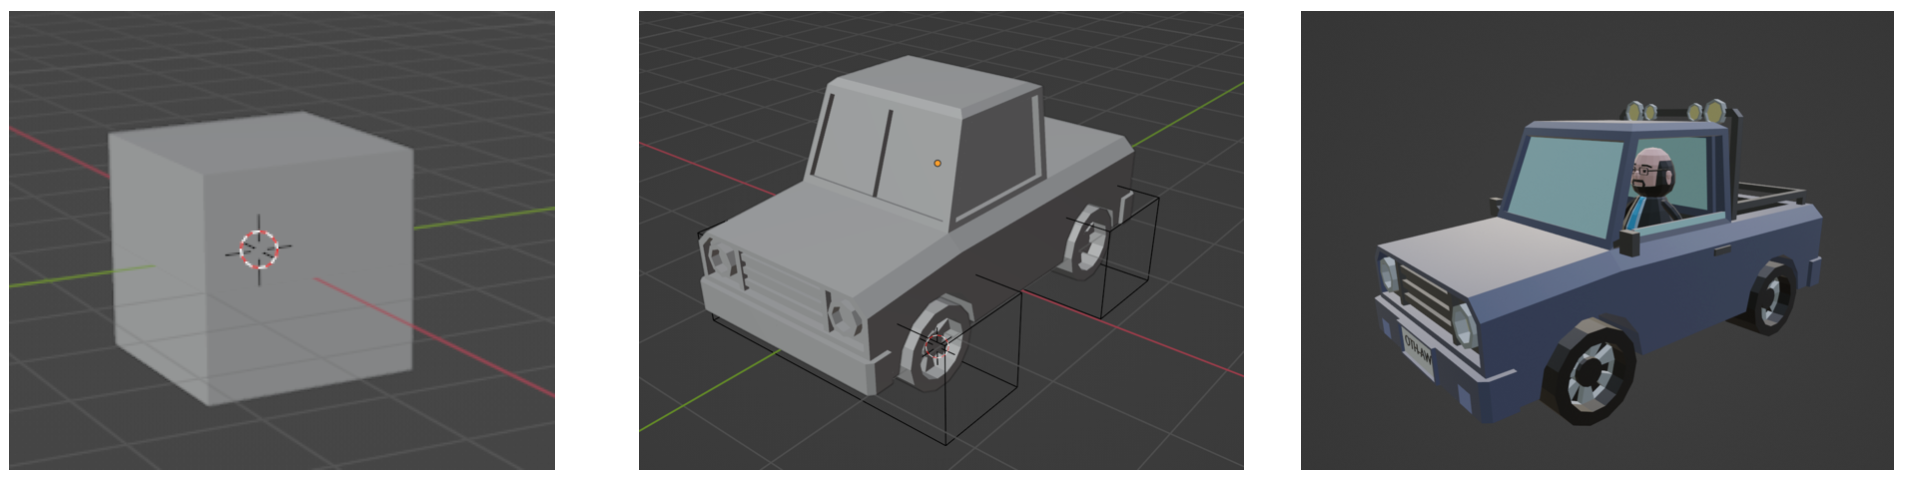
\includegraphics[width=0.8\linewidth]{Development_Pickup.png}
	\caption[Entwicklungsprozess des Pickups mit Blender]{Entwicklungsprozess des Pickups mit Blender. Links: Ausgangsobjekt, Mitte: Zwischenstand, Rechts: Fertige Objekt. Quelle: Eigene Aufnahme}
	\label{fig:development_pickup}
\end{figure}

Mithilfe der 3D-Objektmodellierungssoftware Blender wurden die in \autoref{fig:development_car} und \ref{fig:development_pickup} abgebildeten Objekte erstellt. Ausgehend von dem Würfel sind die Autos Stückweise mit den Werkzeugen (Extrude, Cut, Scale, ...) von Blender erweitert worden. Als Abschluss werden die Materialien für die Texturen der Objekte erstellt.

Im Endprozess kann man mithilfe von Keyframes in Blender die Animationen festlegen. Die Reifen werden mit einer einfachen Rotationsbewegung über eine Zeitspanne verändert. Für die Wink-Bewegung des Charakters im Auto ist auf die Möglichkeiten der Knochen zurückgegriffen worden. Den Körper können eine beliebige Anzahl an Knochen gegeben werden. Diese fungieren wie Gelenke und können anschließend in den Keyframes zu den jeweiligen Zeitpunkten beliebig verändert werden.

\begin{figure}[H]
	\centering
	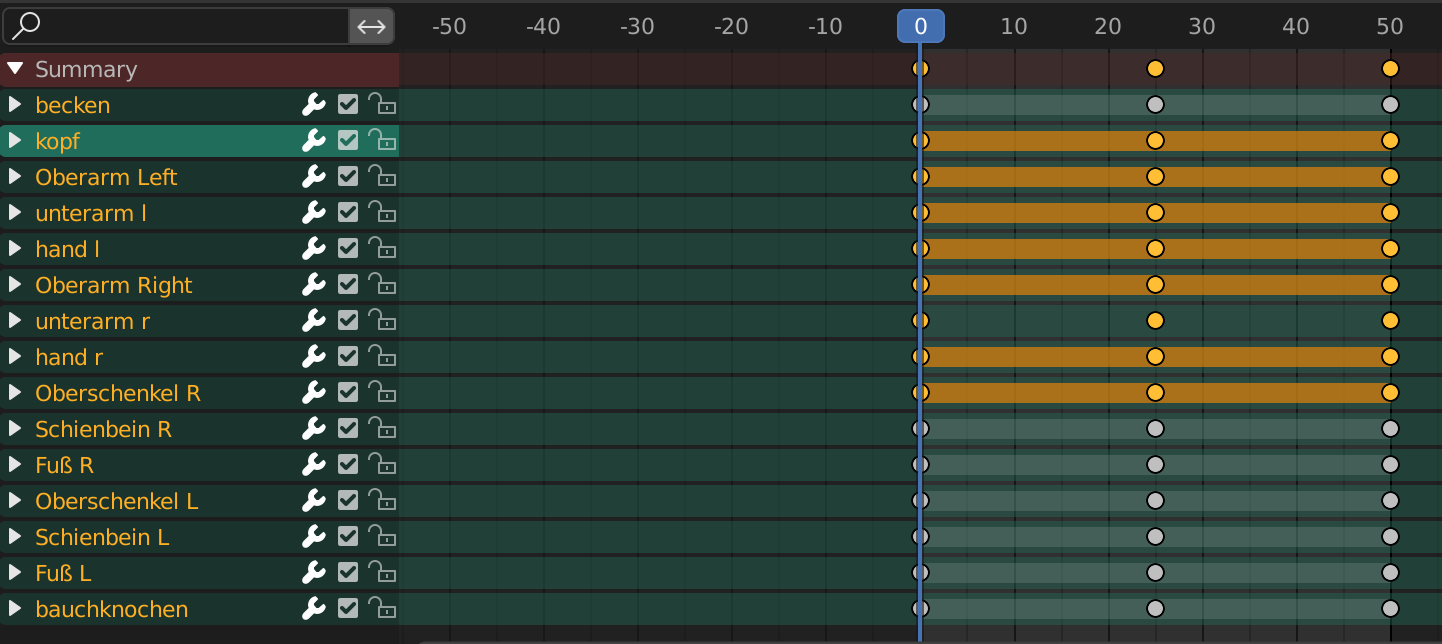
\includegraphics[width=0.5\linewidth]{Keyframes_Animation.png}
	\caption[Keyframes Animation]{Keyframes Animation. Quelle: Eigene Aufnahme}
	\label{fig:keyframes_animation}
\end{figure}

Nach dem Exportieren des fertigen Objekts werden in Unity mithilfe von einem Animator die Animationen abgespielt. Für das gleichzeitige Abspielen der 4 Reifen wurde auf einen Blend-Tree zurückgegriffen. Dieser hat es ermöglicht, dass mit seinen festzulegenden Variablen alle Animationen eines Objektes zur selben Zeit abgespielt werden. 


\subsection{Implementierung}
Beide Autos fahren auf der in \autoref{fig:map} unter Punkt 8 befindlichen Station Straße. Gelangt der Spieler zu dieser Station steht er vor einer Frage und muss diese aus 3 Antwortmöglichkeiten richtig beantworten. Wenn diese erfolgreich beantwortet wird, erhält der Spieler ein weiteres Blatt als Belohnung.

Als kleines Easter-Egg wurde in den Pickup das Asset des Professors Pirkl als Fahrer eingesetzt. Blickt man auf die Straße erkennt man, wie der Fahrer an einem vorbeifährt und dabei aus dem Auto winkt. Das Asset wurde netterweise von Dominik Schweiger zur Verfügung gestellt. Dieser ist angehöriger der Gruppe, die dieses für eine Projektarbeit erstellt haben.


\section{Station 4: Zaun}
Um das Blatt bei dieser Station zu erlangen, muss der Igel der im Zaun feststeckt befreit werden. Dies geschieht, indem der Spieler den Igel mit seinem Controller herauszieht. Für diese 3 unterschiedlichen Zustände existieren 3 Animationen. Abhängig von der Aktion muss eine von diesen ausgeführt werden. Die Schnittstelle zu dem Aufrufen der Aktionen sind in einem Skript implementiert worden. Johannes Horst musste nur noch eine der Funktionen abhängig von seiner ausgeführten Aktion mit dem Controller ausführen.

\section{Spielende}
Für die Registrierung des Spielendes wird ein Event ausgelöst, wenn alle 8 Blätter eingesammelt wurden. Dieses Event triggert eine Funktion und setzt ein Flag auf True. Mithilfe der Basisklasse der Station (Skript von Stefanie Hofmann entwickelt) kann die Position des Spielers abgefragt werden. Wenn dieser sich nach erfolgreichen Beendigen aller Aufgaben im Haus wieder einfindet, ist das Spiel geschafft und die Szene wechselt zu den Credits.



